% Options for packages loaded elsewhere
\PassOptionsToPackage{unicode}{hyperref}
\PassOptionsToPackage{hyphens}{url}
%
\documentclass[
  12pt,
]{article}
\usepackage{lmodern}
\usepackage{amssymb,amsmath}
\usepackage{ifxetex,ifluatex}
\ifnum 0\ifxetex 1\fi\ifluatex 1\fi=0 % if pdftex
  \usepackage[T1]{fontenc}
  \usepackage[utf8]{inputenc}
  \usepackage{textcomp} % provide euro and other symbols
\else % if luatex or xetex
  \usepackage{unicode-math}
  \defaultfontfeatures{Scale=MatchLowercase}
  \defaultfontfeatures[\rmfamily]{Ligatures=TeX,Scale=1}
  \setmainfont[]{Times New Roman}
\fi
% Use upquote if available, for straight quotes in verbatim environments
\IfFileExists{upquote.sty}{\usepackage{upquote}}{}
\IfFileExists{microtype.sty}{% use microtype if available
  \usepackage[]{microtype}
  \UseMicrotypeSet[protrusion]{basicmath} % disable protrusion for tt fonts
}{}
\makeatletter
\@ifundefined{KOMAClassName}{% if non-KOMA class
  \IfFileExists{parskip.sty}{%
    \usepackage{parskip}
  }{% else
    \setlength{\parindent}{0pt}
    \setlength{\parskip}{6pt plus 2pt minus 1pt}}
}{% if KOMA class
  \KOMAoptions{parskip=half}}
\makeatother
\usepackage{xcolor}
\IfFileExists{xurl.sty}{\usepackage{xurl}}{} % add URL line breaks if available
\IfFileExists{bookmark.sty}{\usepackage{bookmark}}{\usepackage{hyperref}}
\hypersetup{
  pdftitle={Comparison of Effects of COVID-19 on Counties With and Without Coal Mines},
  pdfauthor={Thomas Hancock},
  hidelinks,
  pdfcreator={LaTeX via pandoc}}
\urlstyle{same} % disable monospaced font for URLs
\usepackage[margin=2.54cm]{geometry}
\usepackage{longtable,booktabs}
% Correct order of tables after \paragraph or \subparagraph
\usepackage{etoolbox}
\makeatletter
\patchcmd\longtable{\par}{\if@noskipsec\mbox{}\fi\par}{}{}
\makeatother
% Allow footnotes in longtable head/foot
\IfFileExists{footnotehyper.sty}{\usepackage{footnotehyper}}{\usepackage{footnote}}
\makesavenoteenv{longtable}
\usepackage{graphicx,grffile}
\makeatletter
\def\maxwidth{\ifdim\Gin@nat@width>\linewidth\linewidth\else\Gin@nat@width\fi}
\def\maxheight{\ifdim\Gin@nat@height>\textheight\textheight\else\Gin@nat@height\fi}
\makeatother
% Scale images if necessary, so that they will not overflow the page
% margins by default, and it is still possible to overwrite the defaults
% using explicit options in \includegraphics[width, height, ...]{}
\setkeys{Gin}{width=\maxwidth,height=\maxheight,keepaspectratio}
% Set default figure placement to htbp
\makeatletter
\def\fps@figure{htbp}
\makeatother
\setlength{\emergencystretch}{3em} % prevent overfull lines
\providecommand{\tightlist}{%
  \setlength{\itemsep}{0pt}\setlength{\parskip}{0pt}}
\setcounter{secnumdepth}{5}

\title{Comparison of Effects of COVID-19 on Counties With and Without Coal
Mines}
\usepackage{etoolbox}
\makeatletter
\providecommand{\subtitle}[1]{% add subtitle to \maketitle
  \apptocmd{\@title}{\par {\large #1 \par}}{}{}
}
\makeatother
\subtitle{\url{https://github.com/tnh2/ENV872_Project}}
\author{Thomas Hancock}
\date{}

\begin{document}
\maketitle

\newpage
\tableofcontents 
\newpage
\listoftables 
\newpage
\listoffigures 
\newpage

\hypertarget{rationale-and-research-questions}{%
\section{Rationale and Research
Questions}\label{rationale-and-research-questions}}

The purpose of this analysis is to explore whether counties with coal
mines are impacted differently by COVID-19. With the novel coronavirus
rapidly spreading through the United States, different locations are
likely to be affected in different ways. In order to perform the
analysis, I combined datasets containing information about coal mine
locations, populations, and COVID-19 cases and deaths at the county
level. Because other factors such as socioeconomic levels, population
densities, and even government responses to the COVID-19 crisis vary
widely across states, I decided that it was best to compare counties
within states rather than performing analysis on the entire country. In
particular, I focused on Pennsylvania and West Virginia. Pennsylvania
has had a relatively large number of confirmed COVID-19 cases, meaning
there is a reasonable amount of data to analyze. West Virginia has had
relatively few confirmed cases, but I included it as a comparison to
Pennsylvania since West Virginia coal mines have continued operation
whereas Pennsylvania mines were closed in March\textsuperscript{1}.

I am particularly interested in whether or not there will be a
difference in COVID-19 fatality (the percentage of people who have the
disease that die from it) between the counties with coal mines and those
without. The rational behind this exploration is that COVID-19 seems to
be particularly lethal among people with existing conditions, especially
respiratory issues. In turn, coal miners frequently suffer respiratory
issues from the large amonts of dust that they encounter in their jobs.
As such, I wondered if there might be a higher fatality rate in coal
mining counties than non-coal mining counties (as a proxy for fatality
amongst coal miners versus others). Likewise, coal mining involves
sustained close-quarters operation and minimal opportunity for
sanitization. These factors make coal mines a potential hotbed for
COVID-19 spread, leading me to compare counties in Pennsylvania where
the mines shut down in response to the outbreak against counties in West
Virginia where mines continued operation.

My research questions are:

\begin{enumerate}
\def\labelenumi{\arabic{enumi}.}
\item
  Do counties with coal mines have different fatality rates than similar
  counties without coal mines in the same state?
\item
  Do counties with coal mines in Pennsylvania have different fatality
  rates than West Virgnia counties with coal mines?
\end{enumerate}

\newpage

\hypertarget{dataset-information}{%
\section{Dataset Information}\label{dataset-information}}

To perform my analysis, I gathered together five datasets: US Census
state and county boundaries (as shapefiles), US Census population data
for US counties, coal mine locations from the US Department of Energy
(as a shapefile), and county-level COVID-19 case and death counts from
the Johns Hopkins University Center for Systems Science and Engineering
(CSSE). The population data from the US Census Bureau are from 2019
estimates. The coal mine information inlcudes all operating surface and
underground mines in the United States. While the dataset includes
information on the mine type and output, I only used the location data
for this analysis. The COVID-19 data from Johns Hopkins includes
confirmed COVID-19 cases and reported deaths by county as of April 23rd,
2020.

I started wrangling my data by finding which counties had coal mines in
them using the geospatial analysis capabilities of the sf package in R.
I then joined the COVID-19 data with the census population data using
the county FIPS codes and calculated metrics for COVID-19 case rates
(per 100,000 people), fatality rate (deaths per confirmed COVID-19
case), and death rates per 100,000 people in the county. This data was
then combined with the data above identifying whether a county had coal
mines or not to complete the data joining. From this country-wide
dataset, I filtered out the data specific to the two states I focused on
for this study (Pennsylvania and West Virginia). The important data
included in these data sets are outlined in Table 1 below.

\begin{longtable}[]{@{}lll@{}}
\caption{Important Data Fields}\tabularnewline
\toprule
Field Name & Description & Units\tabularnewline
\midrule
\endfirsthead
\toprule
Field Name & Description & Units\tabularnewline
\midrule
\endhead
STNAME & State Name &\tabularnewline
CTYNAME & County Name &\tabularnewline
POPESTIMATE2019 & 2019 Estimated Population & People\tabularnewline
FIPS & 5-digit county identifier &\tabularnewline
Confirmed & Confirmed COVID-19 cases & Total Cases\tabularnewline
Deaths & Reported COVID-19 deaths & Total Deaths\tabularnewline
case\_rate & Rate of COVID-19 cases & Cases per 100,000
people\tabularnewline
death\_rate\_conf & Fatality & Deaths per confirmed case\tabularnewline
death\_rate\_pop & Deaths rate in population & Deaths per 100,000
people\tabularnewline
Mines.Label & Whether the County has mines & Mines or No
Mines\tabularnewline
\bottomrule
\end{longtable}

\newpage

\hypertarget{exploratory-analysis}{%
\section{Exploratory Analysis}\label{exploratory-analysis}}

\hypertarget{pennsylvania-data}{%
\subsection{Pennsylvania Data}\label{pennsylvania-data}}

Turning my attention to Pennsylvania, I started by creating a histogram
of the fatality rates of the coal counties and the non-coal counties.
The first histogram I created is shown in Figure 1 below.

\begin{figure}
\centering
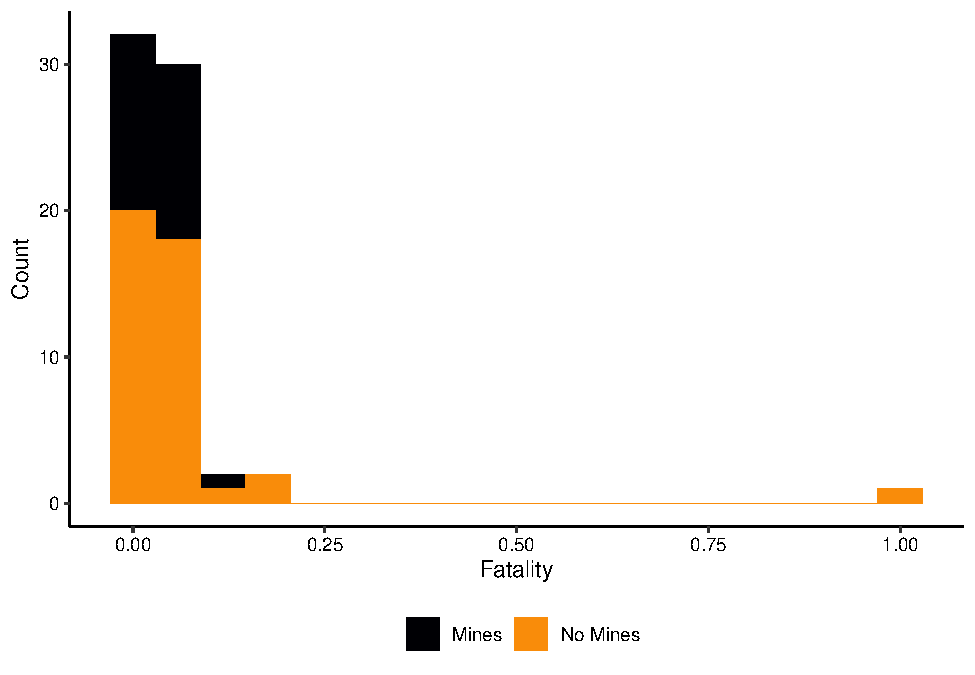
\includegraphics{Hancock_ENV872_Project_files/figure-latex/PA Histogram1-1.pdf}
\caption{Histogram of Fatality in Pennsylvania counties}
\end{figure}

Two things are immediately evident: the data are not normally
distributed, and there are some strange cases where the fatality is 1
(i.e., every confirmed case of COVID-19 resulted in a death). Based on
general knowledge that COVID-19 is not likely to be lethal enough to
kill even a majority of patients, I assumed that these counties had such
limited testing that only the mortalities were tested. For the sake of
this analysis, discarded those counties and any others that have a
fatality rate greater than 50\%. I assumed that the remaining counties
had testing that was sufficiently widespread to provide a reasonable
approximation of the fatality. This new dataset yields the histogram in
Figure 2. The distribution is still not normal, but it has a smoother
shape for both the counties with mines and those without. There are
still a few counties with suspiciously higher fatality rates, but
without further data, there is not enough reason to remove them.

\begin{figure}
\centering
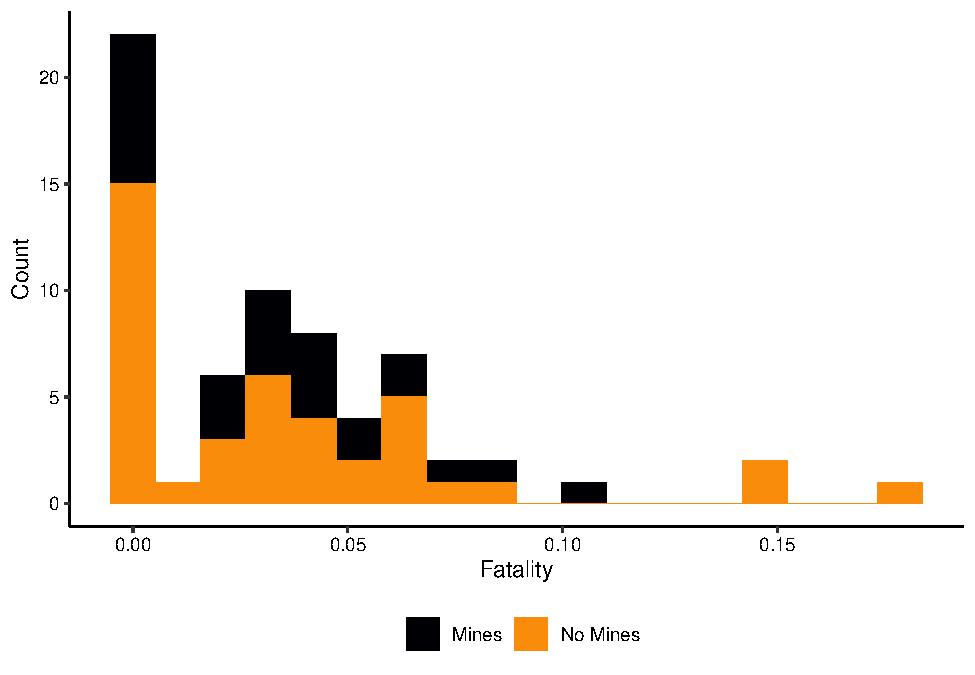
\includegraphics{Hancock_ENV872_Project_files/figure-latex/PA Histogram2-1.pdf}
\caption{Histogram of Fatality in Pennsylvania counties (outliers
removed)}
\end{figure}

I decided to explore the potential relationship between fatality and the
amount of testing by plotting fatality against the number of confirmed
cases per 100,000 people in each county. The results are presented in
Figure 3. Even without the aforementioned counties that only tested
fatal cases, there appears to be a slight decreasing trend in fatality
as the confirmed case rate increases. However, this trend is not
statistically significant (linear regression; p-value = 0.395;
F-statistic = 0.7344; degrees of freedom: 1 and 64).

\begin{figure}
\centering
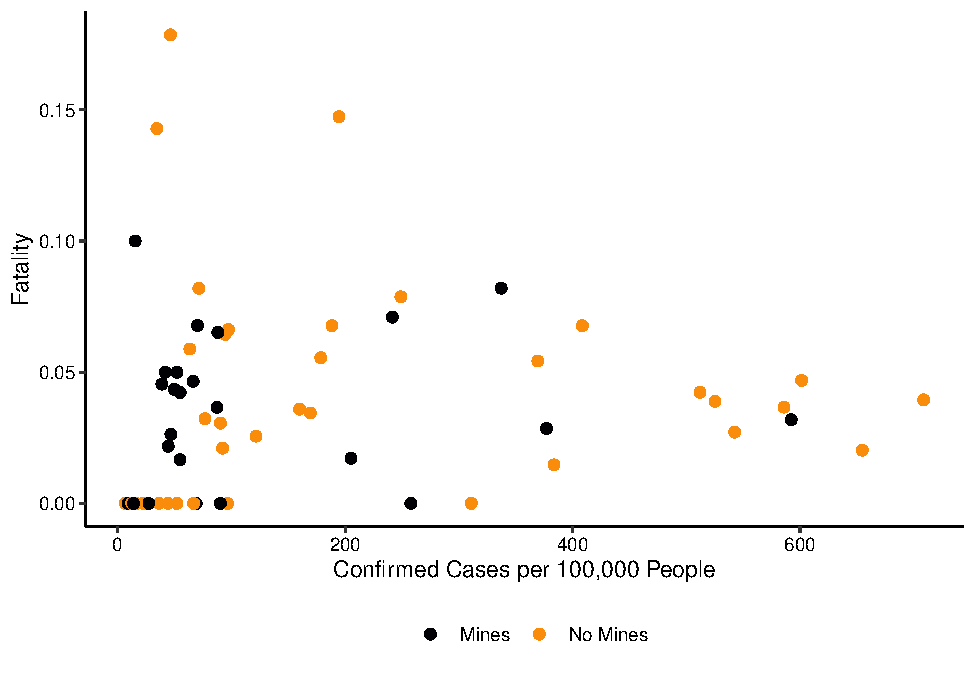
\includegraphics{Hancock_ENV872_Project_files/figure-latex/PA Fatality vs Case Rate-1.pdf}
\caption{Fatality vs confirmed COVID-19 case rate for Pennsylvanian
counties with and without coal mines.}
\end{figure}

\hypertarget{west-virginia-data}{%
\subsection{West Virginia Data}\label{west-virginia-data}}

As mentioned earlier, I am also interested in seeing if there is a
difference between West Virginia, where coal mines stayed open despite
the pandemic, and Pennsylvania, where mines were closed. In Figure 4, I
plotted histograms for the West Virginia data, similar to what was done
for Pennsylvania. From these histograms, one can see that there were a
few West Virignia counties that tested mostly fatal cases of COVID-19,
so it is reasonable to perform the same removal of ouliers with fatality
rates above 50\%. Likewise, the West Virginia data has a very non-normal
distribution.

\begin{figure}
\centering
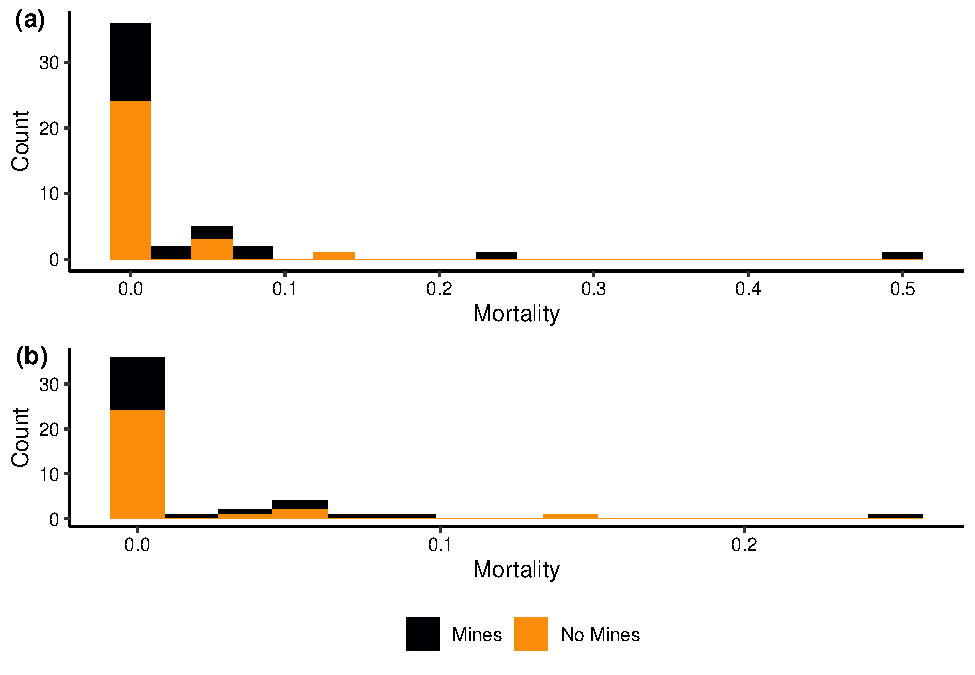
\includegraphics{Hancock_ENV872_Project_files/figure-latex/WV Histograms-1.pdf}
\caption{Histogram of Fatality in West Virginia Counties (a) with
outliers and (b) without outliers.}
\end{figure}

Plotting the fatality against the confirmed case rate for West Virginia
counties, as shown in Figure 5, reveals little structure to the data.
Perhaps the most useful conclusion that can come from this exploration
of the data is that West Virginia has a rather low reported case rate.

\begin{figure}
\centering
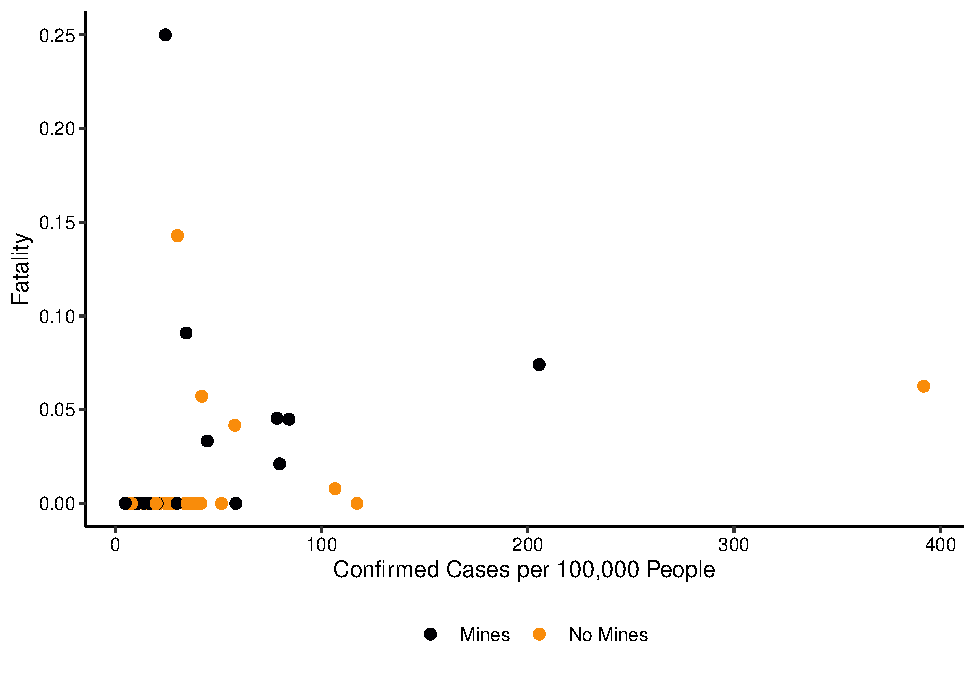
\includegraphics{Hancock_ENV872_Project_files/figure-latex/WV Fatality vs Case Rate-1.pdf}
\caption{Fatality vs confirmed COVID-19 case rate for West Virginian
counties with and without coal mines.}
\end{figure}

\newpage

\hypertarget{analysis}{%
\section{Analysis}\label{analysis}}

\hypertarget{question-1-do-counties-with-coal-mines-have-different-fatality-rates-than-similar-counties-without-coal-mines-in-the-same-state}{%
\subsection{Question 1: Do counties with coal mines have different
fatality rates than similar counties without coal mines in the same
state?}\label{question-1-do-counties-with-coal-mines-have-different-fatality-rates-than-similar-counties-without-coal-mines-in-the-same-state}}

To answer the first question comparing coal mining counties in
Pennsylvania to non-mining counties, I performed a non-parametric
Wilcoxon rank sum test. I chose to use a non-parametric test because the
data are not distributed normally (as seen in the Exploration section).
The Wilcoxon test uses a ranking system to see if two data sets come
from the same distribution. According to this test, there is no
significant difference between the fatality rates in coal mining
counties versus non-mine counties (Wilcoxon test; p = 0.7516; W =
536.5). To visualize this result, I made a boxplot for both sets of data
(fatality in each type of county). This boxplot is shown in Figure 6.
The similarity between the two boxplots reinforces the fact that the two
sets of data are similar.

\begin{figure}
\centering
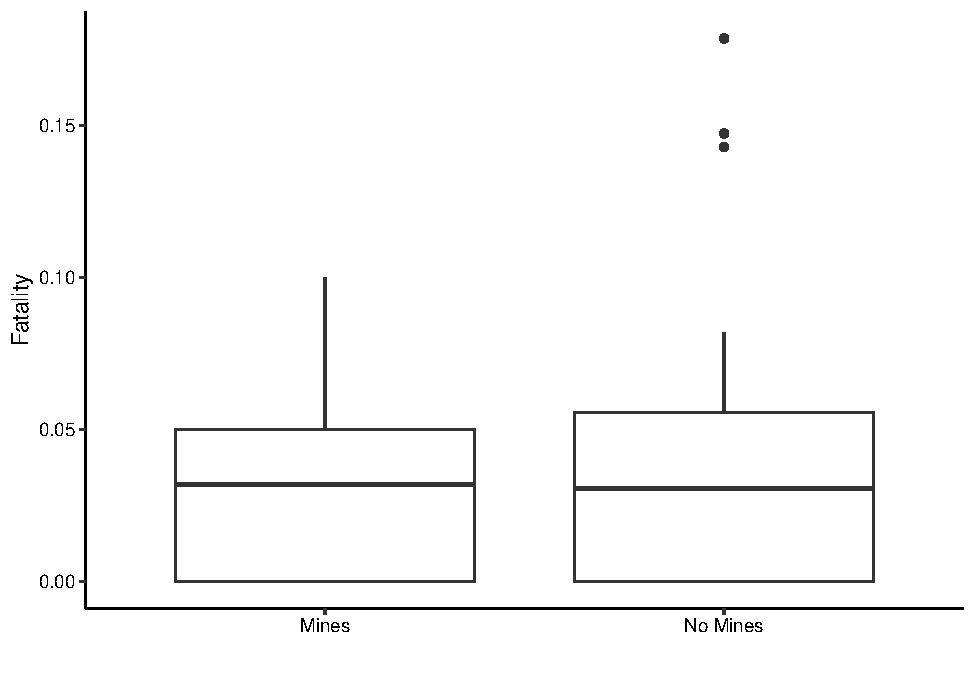
\includegraphics{Hancock_ENV872_Project_files/figure-latex/PA_Boxplots-1.pdf}
\caption{Boxplots of fatality in Pennsylvania counties.}
\end{figure}

\hypertarget{question-2-do-counties-with-coal-mines-in-pennsylvania-have-different-fatality-rates-than-west-virgnia-counties-with-coal-mines}{%
\subsection{Question 2: Do counties with coal mines in Pennsylvania have
different fatality rates than West Virgnia counties with coal
mines?}\label{question-2-do-counties-with-coal-mines-in-pennsylvania-have-different-fatality-rates-than-west-virgnia-counties-with-coal-mines}}

I also used a Wilcoxon test for the second question. As with the first
question, the West Virginia and Pennsylvania mine counties have
non-normal distributions. Once again, there is no significant difference
between the fatality cases in the mining counties of the two states
(Wilcoxon Test; p = 0.0905; W = 306.5). Boxplots of the fatality rates
in the two states also show that they are not significantly different
(Figure 7).

\begin{figure}
\centering
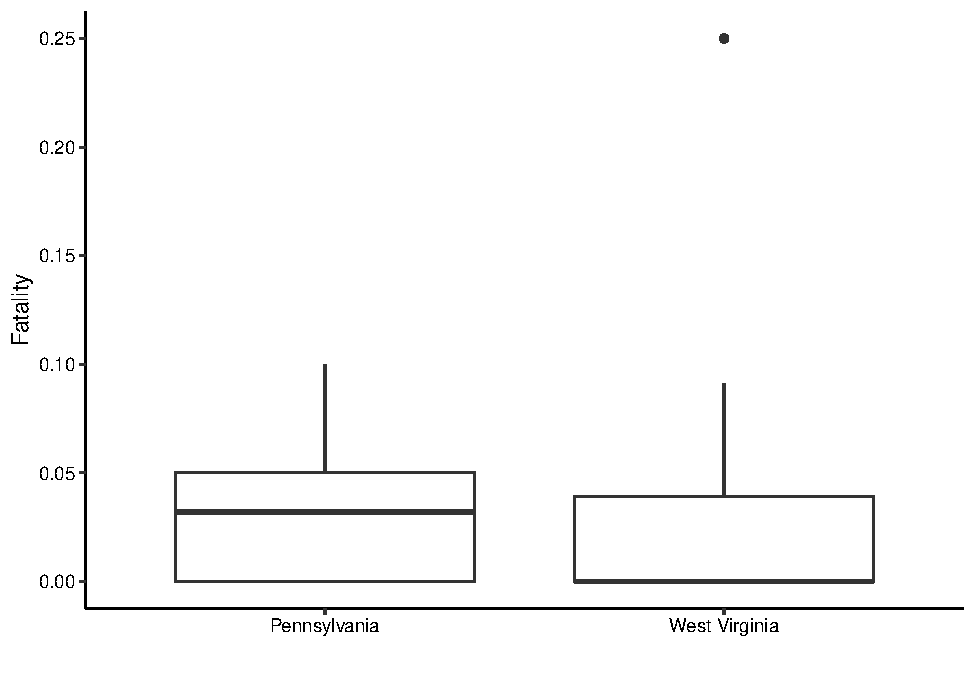
\includegraphics{Hancock_ENV872_Project_files/figure-latex/PA-WV_Boxplots-1.pdf}
\caption{Boxplots of fatality in mining counties in Pennsylvania and
West Virginia.}
\end{figure}

\newpage

\hypertarget{summary-and-conclusions}{%
\section{Summary and Conclusions}\label{summary-and-conclusions}}

Based on the analyses explained earlier, there does not appear to be a
statistically significant difference in COVID-19 effects on counties
with and without coal mines (in Pennsylvania and West Virginia, at
least). Similarly, the fact that Pennsylvania closed their coal mines
due to the pandemic and West Virginia did not does not seem to have led
to a higher fatality rate in West Virginia. My initial thought was that
counties with coal mines might have higher fatality rates because of the
more severe outcomes associated with COVID-19 in patients with
pre-existing conditions and the prevalence of pulmonary disease among
coal miners. However, there are a number of factors that could account
for this data not yielding these results.

One possibility is that it is too early in the US pandemic to see enough
cases to accurately assess mortality. Especially in West Virginia and
more rural parts of Pennsylvania, there has not been thorough testing,
so the data might not have enough statistical power. Moreover, the virus
might not have infected enough people in these regions yet to be able to
compare the outcomes. It is possible that, as the virus spreads, more
cases (and, subsequently, more fatality data) will become available.
Perhaps by the end of this summer, a similar analysis might have a
different outcome. Conversely, it is possible that the virus will not
impact these regions as much as expected. A number of theories have been
proposed for why this low incidence might be observed, including the
fact that these smaller communities tend to be more spread out (so the
virus spreads slower) or that the virus has actually been in West
Virginia longer than is commonly thought (potentially since December).
Even if there is truth to these ideas, it seems very likely that a major
limitation of this study is limited testing, which results in a lack of
data.

Another factor that might have led to these negative results is that the
number of mining community members who are actually miners is often
quite low (especially at the county level). As such, the number of
people in the county who are actually compromised because of the
presence of the mine is relatively low. Socioeconomic factors, or even
potential vulnerabilities due to pollution from the mine, can cross
county lines to other non-mining counties, which would lessen the
difference seen when comparing the two.

Nonetheless, it is interesting to see that there is no appreciable
difference bewteen mining and non-mining counties when it comes to
COVID-19 fatalities. Further work could be done to identify factors that
can contribute to differences in fatality (including prevalence of
testing, air quality issues, and socioeconomic factors, among others).
It will also be interesting to see how the COVID-19 situation evolves,
and similar analyses may be warranted in a number of months when more
data is available.

\newpage

\hypertarget{references}{%
\section{References}\label{references}}

\begin{enumerate}
\def\labelenumi{\arabic{enumi}.}
\tightlist
\item
  Smith, J. (2020, April 5). In West Virginia, experts say coal mines
  could be massive spreading ground for COVID-19. Mines across the state
  are still operating normally. \emph{Times West Virginia}, Retrieved
  from www.timeswv.com
\end{enumerate}

\end{document}
